\setchapterpreamble[u]{%
\dictum[Sokrates]{Hast du etwas Schwieriges zu erledigen, beauftrage damit einen Faulen. Er wird einen leichten Weg finden, es auszuführen. \dots}}
\chapter{Aufgabenbeschreibung} \index{Aufgabenbeschreibung}\label{kap:aufgabenbeschreibung}

\section{Problemstellung}\label{sec:problemstellung}\index{Problemstellung}\index{Geschäftsprozesse}
%\todotext{Problemstellung ausformulieren: 
%Was ist das Problem? 
%• Warum ist es wichtig? 
%• Warum ist es nicht trivial? 
%• Was möchte ich zur Lösung beitragen beitragen? 
%}

%Was ist das Problem, aktuelle Situation?
%Automatisierter Datenaustausch von Produktdaten in der Industrie, konkretes Problem Abfrage der Produktdaten und Antwort. 

Der automatisierte Austausch von Produktdaten spielt in der Geschäftswelt eine große Rolle. Es fallen in der Industrie, der Wissenschaft sowie in der Gesellschaft und Verwaltung große Datenmengen an, wie z.B. die Daten von Produkten, Bestellungen, Rechnungen, Lieferungen oder in der Verwaltung von Personen. Diese Datenmengen müssen nicht nur gespeichert sondern auch bereitgestellt respektive ausgetauscht werden. Der elektronische Datenaustausch erfolgt in der Regel nach einem festem Schema. Hierbei ist das Austauschformat sowie die Schnittstelle über die diese Daten ausgetauscht werden dem Anfragenden als auch dem Anbieter bekannt. Man \enquote{einigt} sich auf definierte Schemata. Dafür nutzt man definierte Standards, um \gls{Interoperabel}\footnote{Die Fähigkeit homogener Systeme Informationen effizient auszutauschen.} zu gewährleisten. Zwei Applikationen sind interoperabel, wenn sie die terminologische Semantik in ihren korrespondierenden Konzepten gemeinsam nutzen und teilen \citep[vgl.][S. 23f]{Hemmje}. 
Das bedeutet, dass zwei Parteien, welche die Anforderungen eines Standards bezüglich Schnittstellen erfüllen und entsprechend ihre zu übermittelnden Daten gemäß Schema formen, eben jene Daten miteinander austauschen können. 

Basierend auf diesen Standards werden Geschäftsprozesse definiert, um beispielsweise den Austausch der Daten und somit den Zugriff eines anderen ggfs. entfernten Systems auf diese Daten zu ermöglichen. Diese wohldefinierten Prozesse  der Geschäftswelt sind in der Regel sehr unflexibel. Dadurch, dass das Modell der Daten sowie die Schnittstelle \enquote{fest verdrahtet} sind, bedeuten Änderungen in den Anforderungen bezogen auf Semantik, Struktur und Inhalte der Daten meistens eine Änderung des Modells, gleichsam der auszutauschenden Daten mit ihren Eigenschaften, als auch eine Anpassung der Schnittstelle. Diese Anpassungen sind in der Regel mit hohen Kosten verbunden, denn nicht nur anbieterseitig muss eine Anpassung erfolgen, der Konsument muss häufig über die Änderung informiert sein und seinerseits Anpassungen vornehmen. 
Ferner stellt sich das Problem, dass für komplexere Produktdaten auch komplexe autarke Schnittstellen geschaffen werden müssen, um diese Komplexität zuerst abbilden und schließlich übertragen zu können.  
Folglich ist es wichtig, möglichst flexibel zu sein, gleichzeitig aber auch abstrakte Modelle, welche eine Trennung von Klassenkonzepten und Daten ermöglichen, zu unterstützen. 

Der Anfrage- und Antwortprozess muss automatisierbar respektive maschinenlesbar sein, gleichzeitig fehlerfrei und flexibel \citep[vgl.][]{uiterwykEclass}.

%Beispiele für relationen algebra in latex
%Query \verb$SELECT x.a FROM x,y,z WHERE x.a=y.a OR x.a=z.a$
%$\Pi_{x.a} ((x \Join y)\cup(x \Join z))$.
%$temp1 \leftarrow (customer \times account) $ \\
%$temp2 \leftarrow  \sigma_{(customer.sin = account.sin}(temp1)$ \\
%$basic-cust-accts \leftarrow \Pi_{(name, customer.sin, account-number)} (temp2) $ \\
%$basic-cust-accts \leftarrow \Pi_{(name, customer.sin, account-number)} (\sigma_{customer.sin = account.sin}(customer \times account))$

Um das Problem zu lösen, bieten sich flexible Mechanismen einer \gls{Abfrageschnittstelle} an. Typischerweise ist solch eine \gls{Abfrageschnittstelle} anbieterseitig im Datenbanksystem implementiert. Darauf aufbauend werden für diese Schnittstelle Methoden angeboten, welche diese Abfragen ermöglichen und passend zu diesen Abfragen entsprechende Antworten mit den gewünschten Daten erzeugen. \index{Abfrage- und Antwortschnittstelle}
Diese herkömmlichen Datenaustauschmechanismen eignen sich somit für eine konkrete Schnittstelle, definieren ein Schema zum Datenaustausch und sind eng an das Domänenmodell gekoppelt. Die flexiblen Abfragemechanismen sind anbieterseitig nahe der Datenquelle implementiert, zumeist bereits implizit vorhanden, beispielsweise durch ein Datenbanksystem mit SQL\footnote{Standard Query Language - Abfragesprache für relationale Datenbanken}-Abfrageschnittstelle. \index{SQL}

Wie bereits erwähnt, baut herkömmlicherweise auf eine SQL-Schnittstelle eine Ebene mit Abfragemethoden auf, um den Zugriff für Business Funktionalität einfacher zu ermöglichen. Führt man eine weitere zusätzliche Ebene ein, die mittels eines Schemas eine flexible \gls{Abfrageschnittstelle} darstellt, so ermöglicht diese einen flexiblen und standardisierten Datenaustausch, wobei die tatsächlichen Werte der Daten vom eigentlichen Domänenmodell abgekoppelt sind. Diese lose Kopplung ist der große Vorteil dieser Lösung und ermöglicht eine große Anpassungsflexibilität. Konkret werden Daten über die Eigenschaften eines Produktes übermittelt, allerdings liegt der Nachricht keine Semantik bei. In der Nachricht wird mittels eines eindeutigen Identifiers auf eine \gls{Ontologie} verwiesen. Der Anfragende muss folglich eine weitere \gls{Ontologie}-Quelle abfragen, um Metainformationen über die Bedeutung des erhaltenen Wertes zu erlangen. 
Der Einsatz einer \gls{Ontologie} als Anfrage- und Antwortmodell vereinfacht die Suche und das Browsing von Informationen \citep[vgl.][S. 24f]{Hemmje}.

Mit diesem Problem haben sich bereits mehrere Interessensgruppen befasst, wie z.B. eCl@ss \citep[vgl.][]{uiterwykEclass}. Es gibt einige Standards welche bei der Lösung unterstützen. Zu nennen ist ISO Standard 22745-35 oder ISO Standard 29002-31. Diese beschreiben eine solche Abfrage- und Antwortschnittstelle auf Ontologiebasis. Die Standards zeigen den flexiblen automatisierten Austausch von charakteristischen Produktdaten auf. Diese Daten (meist Master Data) werden abgekoppelt von der Semantik abgefragt. Die Semantik wird mittels Klassenkonzepten beschrieben. Auf diese Klassenkonzepte wird wie bereits vorab beschrieben mittels eindeutigem \glslink{IRDI}{Identifier} referenziert und die konkreten Daten als Schlüssel-Wertepaare hinterlegt. \index{eCl@ss} \index{Ontologie} \index{IRDI}

\section{Zielsetzung}\index{Zielsetzung}\index{Projektion}\index{Selektion}

Ziel der Arbeit ist es eine flexible Abfrageschnittstelle (Query-Schnittstelle) zu implementieren. Als Datenbasis mit notwendigen Katalog-, Klassenkonzept- und Metadaten soll die bereits vorhandene PLIB\footnote{Parts Library - Implementierung nach ISO-13584} des Fachbereiches dienen. 

Für diese Abfrageschnittstelle wird der Standard der ISO 29002-31 implementiert, sowie für deren Nutzung gegebenenfalls weitere nötige Standards. Diese Schnittstelle soll einen automatisierten Datenaustausch ermöglichen und technisch auf den Abfrageprozeduren der Datenbankebene (Katalog- und Klassenkonzeptdaten) basieren. Die Implementierung dieser Prozeduren und des Datenbankschemas ist Teil der Arbeit zweier Kommilitonen (Herr Mende und Herr Loth).
 
Ein weiteres Ziel ist die Machbarkeit und die Integration einer flexiblen \gls{Abfrageschnittstelle}. Als Datenbasis soll hierbei die vorhandene \gls{PLIB} Datenbankimplementierung des Fachbereiches genutzt werden. 

Um das Ziel zu erreichen, soll im Rahmen der Arbeit untersucht werden, welche möglichen sinnvollen Anwendungsfälle sich in der Praxis - basierend auf den zu unterstützenden ISO Standards - ergeben. Dafür ist eine Analyse der Standards nötig, um zu prüfen, ob und in welcher Form die flexiblen Abfragemöglichkeiten unterstützt werden. Wie in \autoref{sec:problemstellung} erwähnt, gibt es auf Datenbankebene oft eine implizite Abfrageschnittstelle, welche in SQL realisiert ist. Es bietet sich daher an, die Möglichkeiten von SQL-Abfragen als Basis für die Untersuchung zu nehmen, und zu prüfen welche Abfragen mit Hilfe des Standards realisiert werden können. 
Betrachtet werden soll die Projektion und die Selektion.

\begin{description}
\item[Projektion] Die Attributbeschränkung gleichsam einer \enquote{Spaltenauwahl} in relationalen Datenbanken. In SQL das \enquote{select} Keyword. In Relationenalgebra:

$ergebnisprojektion \leftarrow  \Pi_{(attribut_1, attribut_2... attribut_n)}(plib)$ \\

\item[Selektion] Schränkt eine Suche mittels Prädikaten auf passende Tupel ein, gleichsam einer \enquote{Zeilenauswahl}. In SQL das \enquote{where} Schlüsselwort samt Mengenoperatoren, wie z.B. \enquote{UND, ODER, NICHT}. In Relationenalgebra:

$ergebnisselektion \leftarrow  \sigma_{(praedikat_1, praedikat_2... praedikat_n})(plib)$ \\

\end{description}

Für die Schnittstelle ist eine prototypische Implementierung zu erstellen. Weiterer Bestandteil der Arbeit ist unter Beachtung der technischen Vorgaben, eine Beschreibung des Auswahlprozesses der Techniken, Plattform, Architektur und Programmiersprachen. Die Vor- und Nachteile der einzelnen Optionen des Auswahlprozesses und weitere Nutzungs-, respektive Erweiterungs- und Integrationsmöglichkeiten der entwickelten Schnittstelle sind zu erläutern. 
Die Entwicklung der Software soll nach einem aktuell üblichen Softwareentwicklungsprozess erfolgen. 

\section{Kontext und Abgrenzung}

\subsection{Gesamtkontext der PLIB Abschlussarbeiten}\index{Gesamtkontext}

Um einen Überblick zu schaffen, in welchem Kontext sich diese Arbeit befindet, wird nachfolgend eine kurze Übersicht über die PLIB Abschlussarbeiten des Fachbereiches gegeben.

%\bild{gesamtkontext_plib}{16cm}{gesamtkontext_plib}{gesamtkontext_plib}

\begin{figure}[htbp]
	\centering
		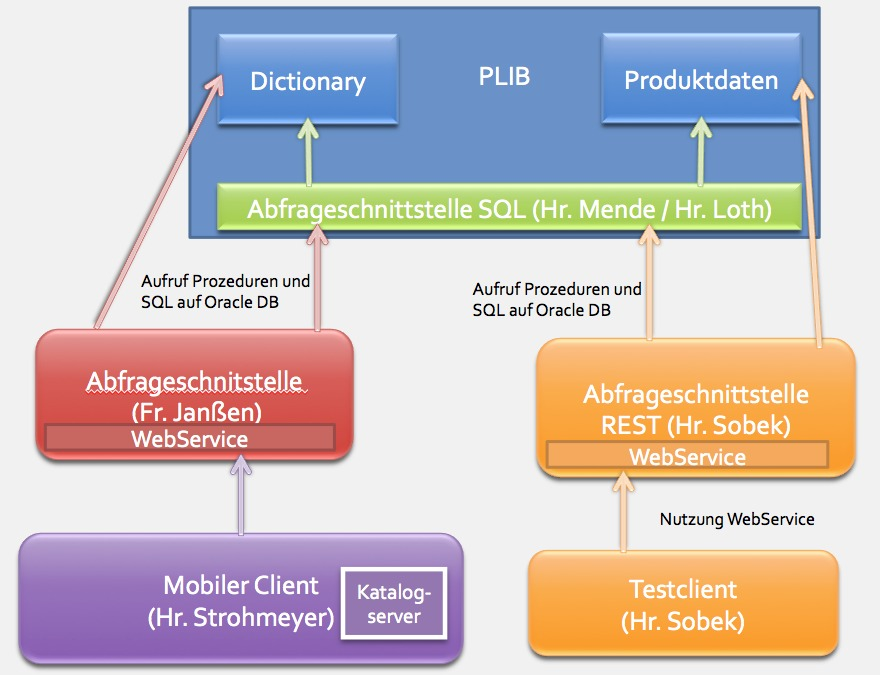
\includegraphics[width=0.75\textwidth]{images/gesamtkontext_plib.jpg}
	\caption{Gesamtkontext PLIB Abschlussarbeiten}
	\label{fig:gesamtkontext_plib}
\end{figure}

Die \autoref{tab.gesamtkontext} erläutert die \autoref{fig:gesamtkontext_plib} und listet dazu die jeweiligen Arbeiten und die zur Problemlösung betrachteten ISO-Standards auf.

% \cellcolor{<Farbe>}, \rowcolor{<Farbe>}, {\columncolor{<Farbe>}}, ändern die Hintergrundfarbe. 
\begin{table}[!hbt]\vspace{1ex}\centering
\scriptsize
\begin{tabular}{p{3cm}p{2.2cm}p{5cm}p{2.6cm}}
\toprule \rowcolor{mylightergray}
\textbf{Bezeichnung} & \textbf{Arbeit von} & \textbf{Erläuterung} &  \textbf{ISO Standards}\\
\midrule
Abfrageschnittstelle als \gls{Webservice} mit \gls{SOAP} &  Frau Janßen & Implementierung eines \glspl{Webservice} zur Auflösung von Konzept-Identifikatoren in Konzept-Dictionaries/Ontologien & ISO 29002-20 \\
\hline
PLIB, Dictionary und Produktdatenbank &  Herr Mende und Herr Loth & Meta- und Produktdatenbank sowie eine Abfrageschnittstelle basierend auf Oracle. Entwicklung von Abfrageschnittstellen mit Oracle Prozeduren & ISO 13584-42 \citep[Vergl.][]{iso13584-42}  \\
\hline
Mobiler Abfrageclient & Herr Lohmeyer & Entwicklung eines mobilen Abfrageclients basierend auf Android. Der Client nutzt die \glspl{Webservice} von Frau Janßen und beinhaltet einen eigenen Katalog\-server. & ISO 29002-10, ISO 13584-42 \\
\hline
Abfrageschnittstelle als \gls{Webservice} mit \gls{REST} für charakteristische Produktdaten & Herr Sobek & Entwicklung einer Schnittstelle zur Abfrage von charakteristischen Produktdaten. Die Schnittstelle wird als \gls{REST}ful \gls{Webservice} implementiert. & ISO 29002-31, ISO 29002-10 \\
\bottomrule
\end{tabular}
\caption{\label{tab.gesamtkontext}Erläuterung der Gesamtkontextabbildung}
\vspace{2ex}\end{table}

\subsection{Abgrenzung} \index{Identification Guide} \index{Abgrenzung} \index{Use Cases}\index{ISO 29002-10}

Die Arbeit umfasst die Implementierung der Use Cases nach \autoref{kap:Use_Cases}. Dies beinhaltet im wesentlichen den Teil 31 der ISO 29002 - einen Abfragestandard für charakteristische Produktdaten. 
Weiterhin wird für die Datenübertragung eine Implementierung des Teils 10 der ISO 29002 benötigt, siehe \autoref{fig:lieferketten}. 
Die Arbeit beinhaltet nicht die Implementierung eines \glspl{IG} nach ISO 22745-30. Dieser wird in der Praxis von einem Klienten für eine sinnvolle Vorauswahl der für sich oder seine Organisation benötigten Attribute der Teile verwendet. Jeder Klient definiert für seinen Kontext sinnvolle Attribute und Teiledaten und definiert diese mit Hilfe des Schemas der ISO 22745-30. Dies kann mittels eines Webformulars auf Klientenseite erfolgen oder als allgemeines Formular mit z.B. \gls{Excel}, welches die für den/die Klienten relevanten Attribute der Produkte, die abgefragt werden sollen, enthält. Für mehr Informationen zum \gls{IG} siehe \autoref{kap:identification_guide}.

%Beispiel: bild mit footnote
\begin{figure}[htbp]
	\centering
		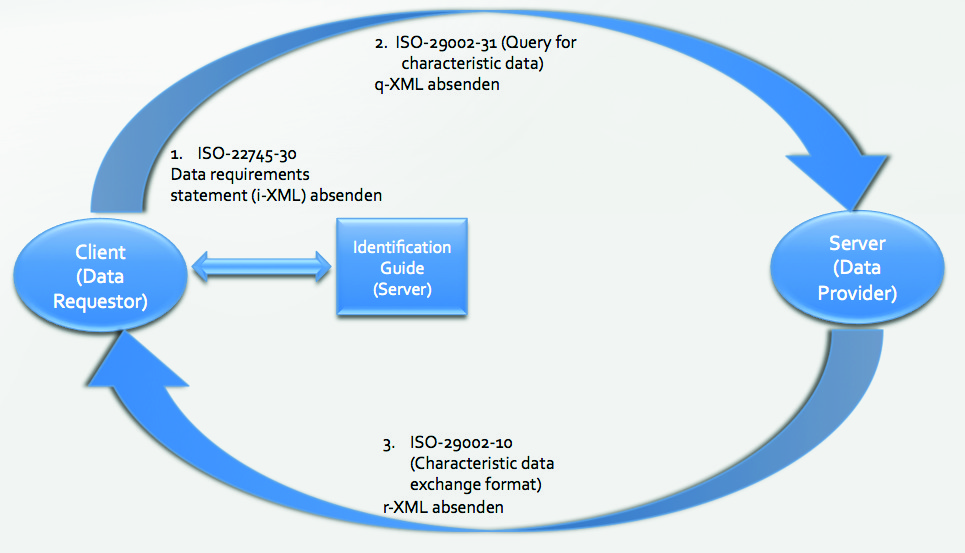
\includegraphics[width=0.90\textwidth]{images/lieferketten_plib.jpg}
		\caption[Lieferketten]{Lieferketten\footnotemark}
	\label{fig:lieferketten}
\end{figure}
\footnotetext{Abbildung entnommen und abgewandelt aus Benson, Converting Standard Terminology into usable Metadata, 2008 - später in ähnlicher Form auch in Uiterwyk, Die Bedeutung der Merkmalleisten bei eCl@ss, 2012 zu finden.}

\subsection{Vorgaben}\index{Vorgaben}\index{Oracle}

Für die Implementierung sind folgende nichtfunktionale Anforderungen vorgegeben:
\begin{description}
\item[Datenbanksystem Oracle] Dieses beinhaltet die PLIB Datenbank samt Abfrageprozeduren und stellt als Teiledatenbank die Basis dar. Dies wird vom Fachbereich bzw. von den Studenten Herr Mende/Herr Loth gestellt.
\item[Webservice] Auf Grund der hohen Verbreitung und Integrationsmöglichkeiten soll die Schnittstelle als \gls{Webservice} entwickelt werden. Die ISO 29002-31 schlägt als Beispiel eine E-Mail-Schnittstelle vor. Siehe \autoref{fig:datenfluesse}, welche besagt:
\begin{quotation}
Transport: not specified in ISO/TS 29002 (could use email) Payload XML.Query XML schema in ISO/TS 29002-31
\end{quotation}
Dies ist folglich nur ein Vorschlag. 
\item[PLIB Datenbankprozeduren] Die vorhandenen Prozeduren zum Zugriff auf die PLIB Datenbank sollen so weit wie möglich verwendet werden. 
\end{description}

\subsection{Datenflüsse} \index{Datenflüsse} \index{Webservice}\index{ISO 29002-10}\index{ISO 29002-31}
Das System soll einen \gls{Webservice} zur Verfügung stellen. Dieser \gls{Webservice} soll eine XML Datei gemäß ISO 29002-31 entgegennehmen. Die entsprechende Verarbeitung des XMLs, sowie die logische Transformation der Anfrage zur Abfrageschnittstelle der Datenbank wird vom System vorgenommen. Die Antwort der Datenbank soll wieder zurücktransformiert werden und als Katalog-XML Datei gemäß ISO 29002-10 zurückgeliefert werden.
 
Der gerahmte Bereich im unteren Teil der \autoref{fig:datenfluesse} zeigt in der Datenflussabbildung, was implementiert werden soll. Das Zielsystem, gleichsam das System, welches die Anfrage erhält, wird hier als \enquote{Catalogue Server} bezeichnet. 
Die Kommunikation des Klienten mit dem Location Server, Terminology Server und dem Ontology Server ist Teil der Abschlussarbeit von Fr. Janßen \citep[Vergl.][]{janssen}. 
Die Abfrageprozeduren des Katalogservers auf Datenbankebene ist Aufgabe von Herrn Mende. Zur Zeit der Abgabe dieser Arbeit, war die Arbeit von Herrn Mende noch in Bearbeitung\footnote{Die Basis dieser Abschlussarbeit ist ein stabiler Implementierungsstand, welcher von Herrn Mende geliefert wurde.}. 

\begin{figure}[htbp]
	\centering
		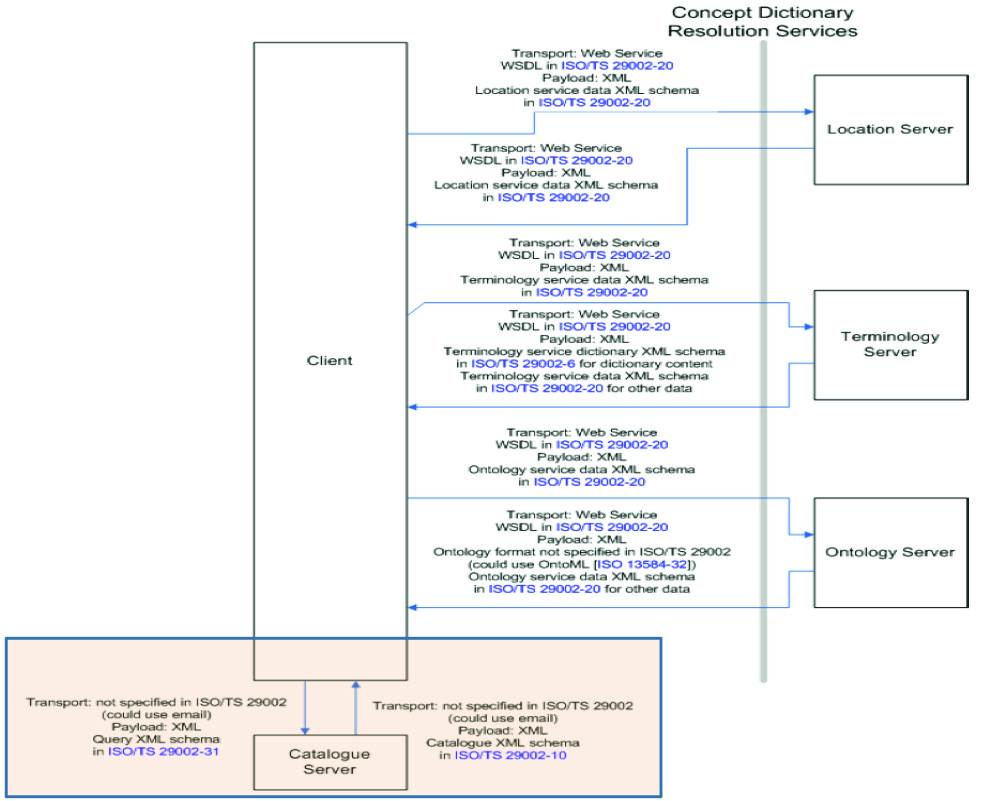
\includegraphics[width=0.90\textwidth]{images/datenfluesse_plib.jpg}
	\caption[Datenflüsse]{Datenflüsse\footnotemark}
	\label{fig:datenfluesse}
\end{figure}
\footnotetext{Quelle: entnommen ISO 29002-31 Figure 3 - Major Dataflows. Zur besseren Visualisierung wurde der untere Bereich farblich hervorgehoben.}
